\section{Desarrollo}

Para resolver el circuito euleriano, debemos recorrer cada arista exactamente una vez,
dado que ya se ha verificado que el circuito es euleriano, podemos proceder a encontrar
una solución.

Para esto empezaremos con un recorrido que inicie en un vértice cualquiera,
por ejemplo, el vértice 0. Desde ahi seleccionamos una de las aristas adyacentes,
buscando recorrer todas hasta lograr un circuito cerrado. Si durante el recorrido
nos encontramos con un vértice que no tiene aristas adyacentes sin recorrer,
entonces debemos retroceder y seleccionar una arista diferente en el paso anterior.
Este proceso se repite hasta que se hayan recorrido todas las aristas del circuito.

\subsection{Aproximación Manual}

Siguiendo el proceso descrito, se puede encontrar una solución manualmente. Partiendo
del vértice 0, se puede seguir el siguiente recorrido:
\begin{center}
  0 $\rightarrow$
  1 $\rightarrow$
  2 $\rightarrow$
  3 $\rightarrow$
  4 $\rightarrow$
  5 $\rightarrow$
  9 $\rightarrow$
  3 $\rightarrow$
  2 $\rightarrow$
  9 $\rightarrow$
  1 $\rightarrow$
  9 $\rightarrow$
  8 $\rightarrow$
  0 $\rightarrow$
  7 $\rightarrow$
  6 $\rightarrow$
  5 $\rightarrow$
  8 $\rightarrow$
  5 $\rightarrow$
  6 $\rightarrow$
  9 $\rightarrow$
  8 $\rightarrow$
  0
\end{center}

\begin{figure}[H]
    \centering
    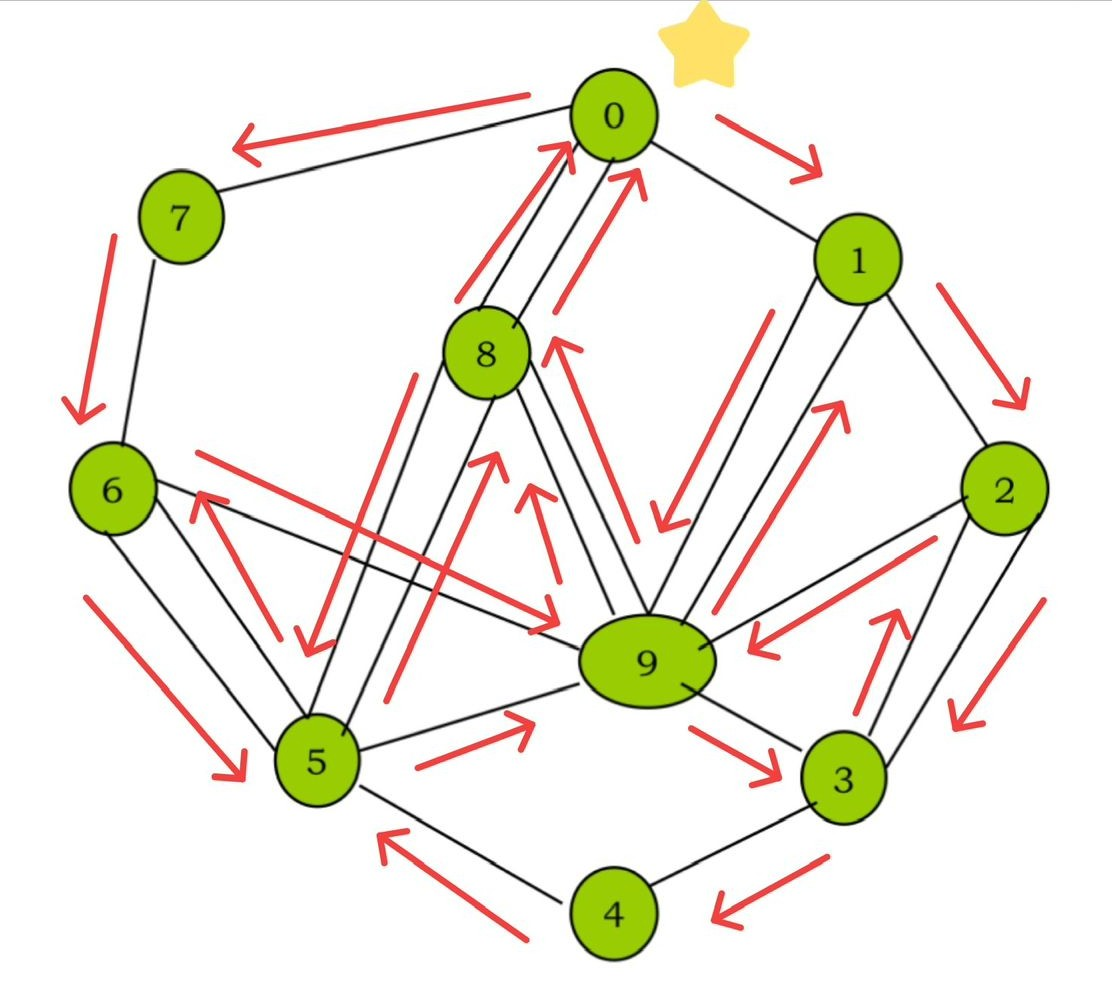
\includegraphics[width=0.6\textwidth]{rsc/img/solucion_manual.jpeg}
    \caption{Recorrido manual del circuito euleriano.}\label{fig:solucion_manual}
\end{figure}

Para esto seguimos el proceso descrito el cual podemos seguir en la siguiente 
Figura~\ref{fig:recorrido_manual_proceso}.

\begin{figure}[H]
    \centering
    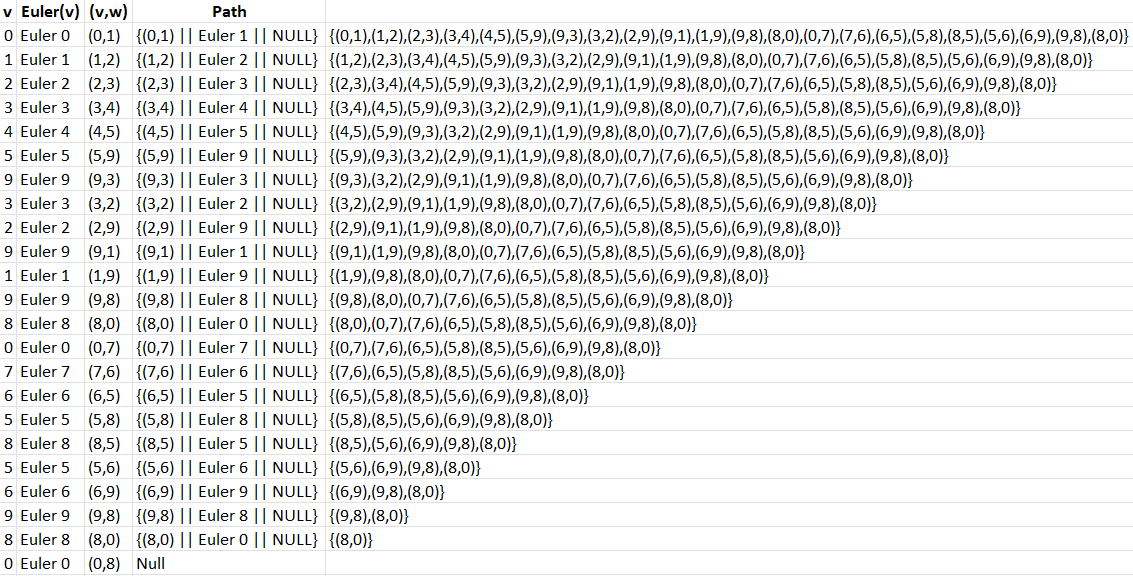
\includegraphics[width=1.1\textwidth]{rsc/img/Tabla.png}
    \caption{Proceso de recorrido manual del circuito euleriano.}\label{fig:recorrido_manual_proceso}
\end{figure}

\subsection{Aproximación Computacional}

Con el codigo visto en clase podemos encontrar una solución computacionalmente.
Una vez que corrimos el programa, obtenemos el siguiente resultado:
\begin{center}
1 $\rightarrow$
9 $\rightarrow$
3 $\rightarrow$
2 $\rightarrow$
3 $\rightarrow$
4 $\rightarrow$
5 $\rightarrow$
9 $\rightarrow$
1 $\rightarrow$
0 $\rightarrow$
8 $\rightarrow$
5 $\rightarrow$
6 $\rightarrow$
5 $\rightarrow$
8 $\rightarrow$
0 $\rightarrow$
7 $\rightarrow$
6 $\rightarrow$
9 $\rightarrow$
8 $\rightarrow$
9 $\rightarrow$
2 $\rightarrow$
1
\end{center}

Como podemos observar, el resultado obtenido computacionalmente es diferente al resultado obtenido 
manualmente, sin embargo, ambos resultados son válidos ya que cumplen con la condición de 
recorrer cada arista exactamente una vez y formar un circuito cerrado. 
Esto demuestra que existen múltiples soluciones para el circuito euleriano dado, y que el 
método utilizado para encontrar una solución puede llevar a diferentes resultados válidos.